\subsection{Solutions to the Euler Equations}
\label{sec:cm1frEuler}
\subsubsection{Setup}

Solving the 1-D Euler equations is a good test of a scheme's robustness and potential for solving challenging Navier-Stokes cases. In this section we compare the performance of \gls{c1fr} to that of unmodified \gls{dg}. The equations in conservative form are

 \begin{equation}\label{1dEuler}
\frac{\partial U}{\partial t} +  \frac{\partial F}{\partial x}  = 0
\end{equation}

where 
\begin{equation}
U = \l(
\begin{tabular}{c}
$\rho$\\
$\rho u$\\
$E$
\end{tabular}
\r), 
\;\;
F = \l(
\begin{tabular}{c}
$\rho u$\\
$\rho u^2 + p$\\
$ u (E + p)$
\end{tabular}
\r), 
\end{equation}

\begin{equation}
E = \l(e + \frac{1}{2}u^2 \r) \rho,
\end{equation}
and 
\begin{equation}
p = (\gamma -1) \l(E - \frac{1}{2}\rho u^2\r).
\end{equation}

$\gamma, \rho, e$ are the usual symbols of ratio of specific heat capacities of the gas, density, and specific internal energy, respectively.

We can rewrite the system of equations so only three variables appear:
\begin{equation}
U = \l(
\begin{tabular}{c}
$U_1$\\
$U_2$\\
$U_3$
\end{tabular}
\r), 
\;\;
F = \l(
\begin{tabular}{c}
$U_2$\\
$\frac{U_2^2}{U_1} + p$\\
$\frac{U_2}{U_1} \l( U_3 + p\r)$
\end{tabular}
\r), \;\;
p = (\gamma - 1)  \l(U_3 - \frac{1}{2} \frac{U_2^2}{U_1}\r)
\end{equation}

It is possible to find exact solutions to problems with initial conditions of the form
\begin{equation*}
\rho(x,0) = \bigg\{
\begin{tabular}{c}
$
\begin{aligned}
\rho_L &\text{ if } x < x_{ref}\\
\rho_R &\text{ if } x \ge x_{ref}
\end{aligned}
$
\end{tabular},
\end{equation*}
\begin{equation}
\label{euler_initConditions}
p(x,0) = \bigg\{
\begin{tabular}{c}
$
\begin{aligned}
p_L &\text{ if } x < x_{ref}\\
p_R &\text{ if } x \ge x_{ref}
\end{aligned}
$
\end{tabular}, \text{ and }
\end{equation}
\begin{equation*}
 u(x,0) =\bigg\{
\begin{tabular}{c}
$
\begin{aligned}
u_L &\text{ if } x < x_{ref}\\
u_R &\text{ if } x \ge x_{ref}
\end{aligned}
$
\end{tabular}.
\end{equation*}
where subscripts $R,L$ mean the value is constant to the right and left, respectively, of the point $x_{ref}$. A thorough description on how to find such exact solutions is in Section 4.2 in \cite{solvers1997numerical}.

High order methods are known to not perform well in the presence of shocks. This is specially true when the initial condition is discontinuous. \gls{c1fr} schemes are not impervious to this problem and become unstable at any \gls{cfl} with discontinuous initial conditions such as those in Eqn. \eqref{euler_initConditions}.

In order to produce a solution, the initial discontinuity is ``thickened'' by using a hyperbolic tangent ($\tanh$) function, as opposed to a Heaviside step function, to step from the left value to the right value. For the following results, 
\begin{equation}
y = \frac{y_R - y_L}{2} \tanh(K (x - x_{ref})) + \frac{y_R + y_L}{2}
\end{equation}

where $y$ is the quantity being initialized ($\rho, p, u$) and $K$ modifies the sharpness of the step. When $K \rightarrow \infty$, we recover the Heaviside step function. A value of $K=90$ produced a subjectively appropriate sharpness and allowed the numerical solution to develop shocks by itself. We are interested in seeing how the numerical scheme handles the latter.

Even though the initial conditions were modified, it is still possible to observe that the \gls{c1fr} functions have enhanced built-in resilience relative to regular \gls{dg}.

No modifications to the interface flux definitions were made for the following results.  It can be argued that a different selection of fluxes and the use of limiters or filters could improve the results of both \gls{c1fr} and \gls{dg}. However, the goal of the following exposition is not to present the ``best'' or a ``better'' numerical scheme for the solution of the Euler equations, but rather to assess the behavior of a general scheme like \gls{c1fr} in a challenging situation that could appear in a flow of engineering interest. The idea behind this goal is that if an untuned scheme performs well in a challenging scenario, it is reasonable to expect the engineer will not need to spend much time and effort tuning the simulation parameters to obtain a useful solution to a problem.

\subsubsection{Results and discussion}
\setcounter{secnumdepth}{5}
\paragraph{Sod's Shock Tube}
\label{sec:shock_tube}
The initial conditions for this problem are, as shown in \cite{roe1981approximate},
\begin{equation*}
\rho(x,0) = \bigg\{
\begin{tabular}{c}
$
\begin{aligned}
1 &\text{ if } x < 0.5\\
0.123 &\text{ if } x \ge 0.5
\end{aligned}
$
\end{tabular},\;\;
p(x,0) = \bigg\{
\begin{tabular}{c}
$
\begin{aligned}
1 &\text{ if } x < 0.5\\
0.1 &\text{ if } x \ge 0.5
\end{aligned}
$
\end{tabular}
,\text{ and } u(x,0) = 0.
\end{equation*}

Figure \ref{c1fr_shockTube_initCond} plots the initial conditions with the ``thickened'' discontinuity.

\begin{figure}
\centering
\hspace{-1.25 cm}
\centering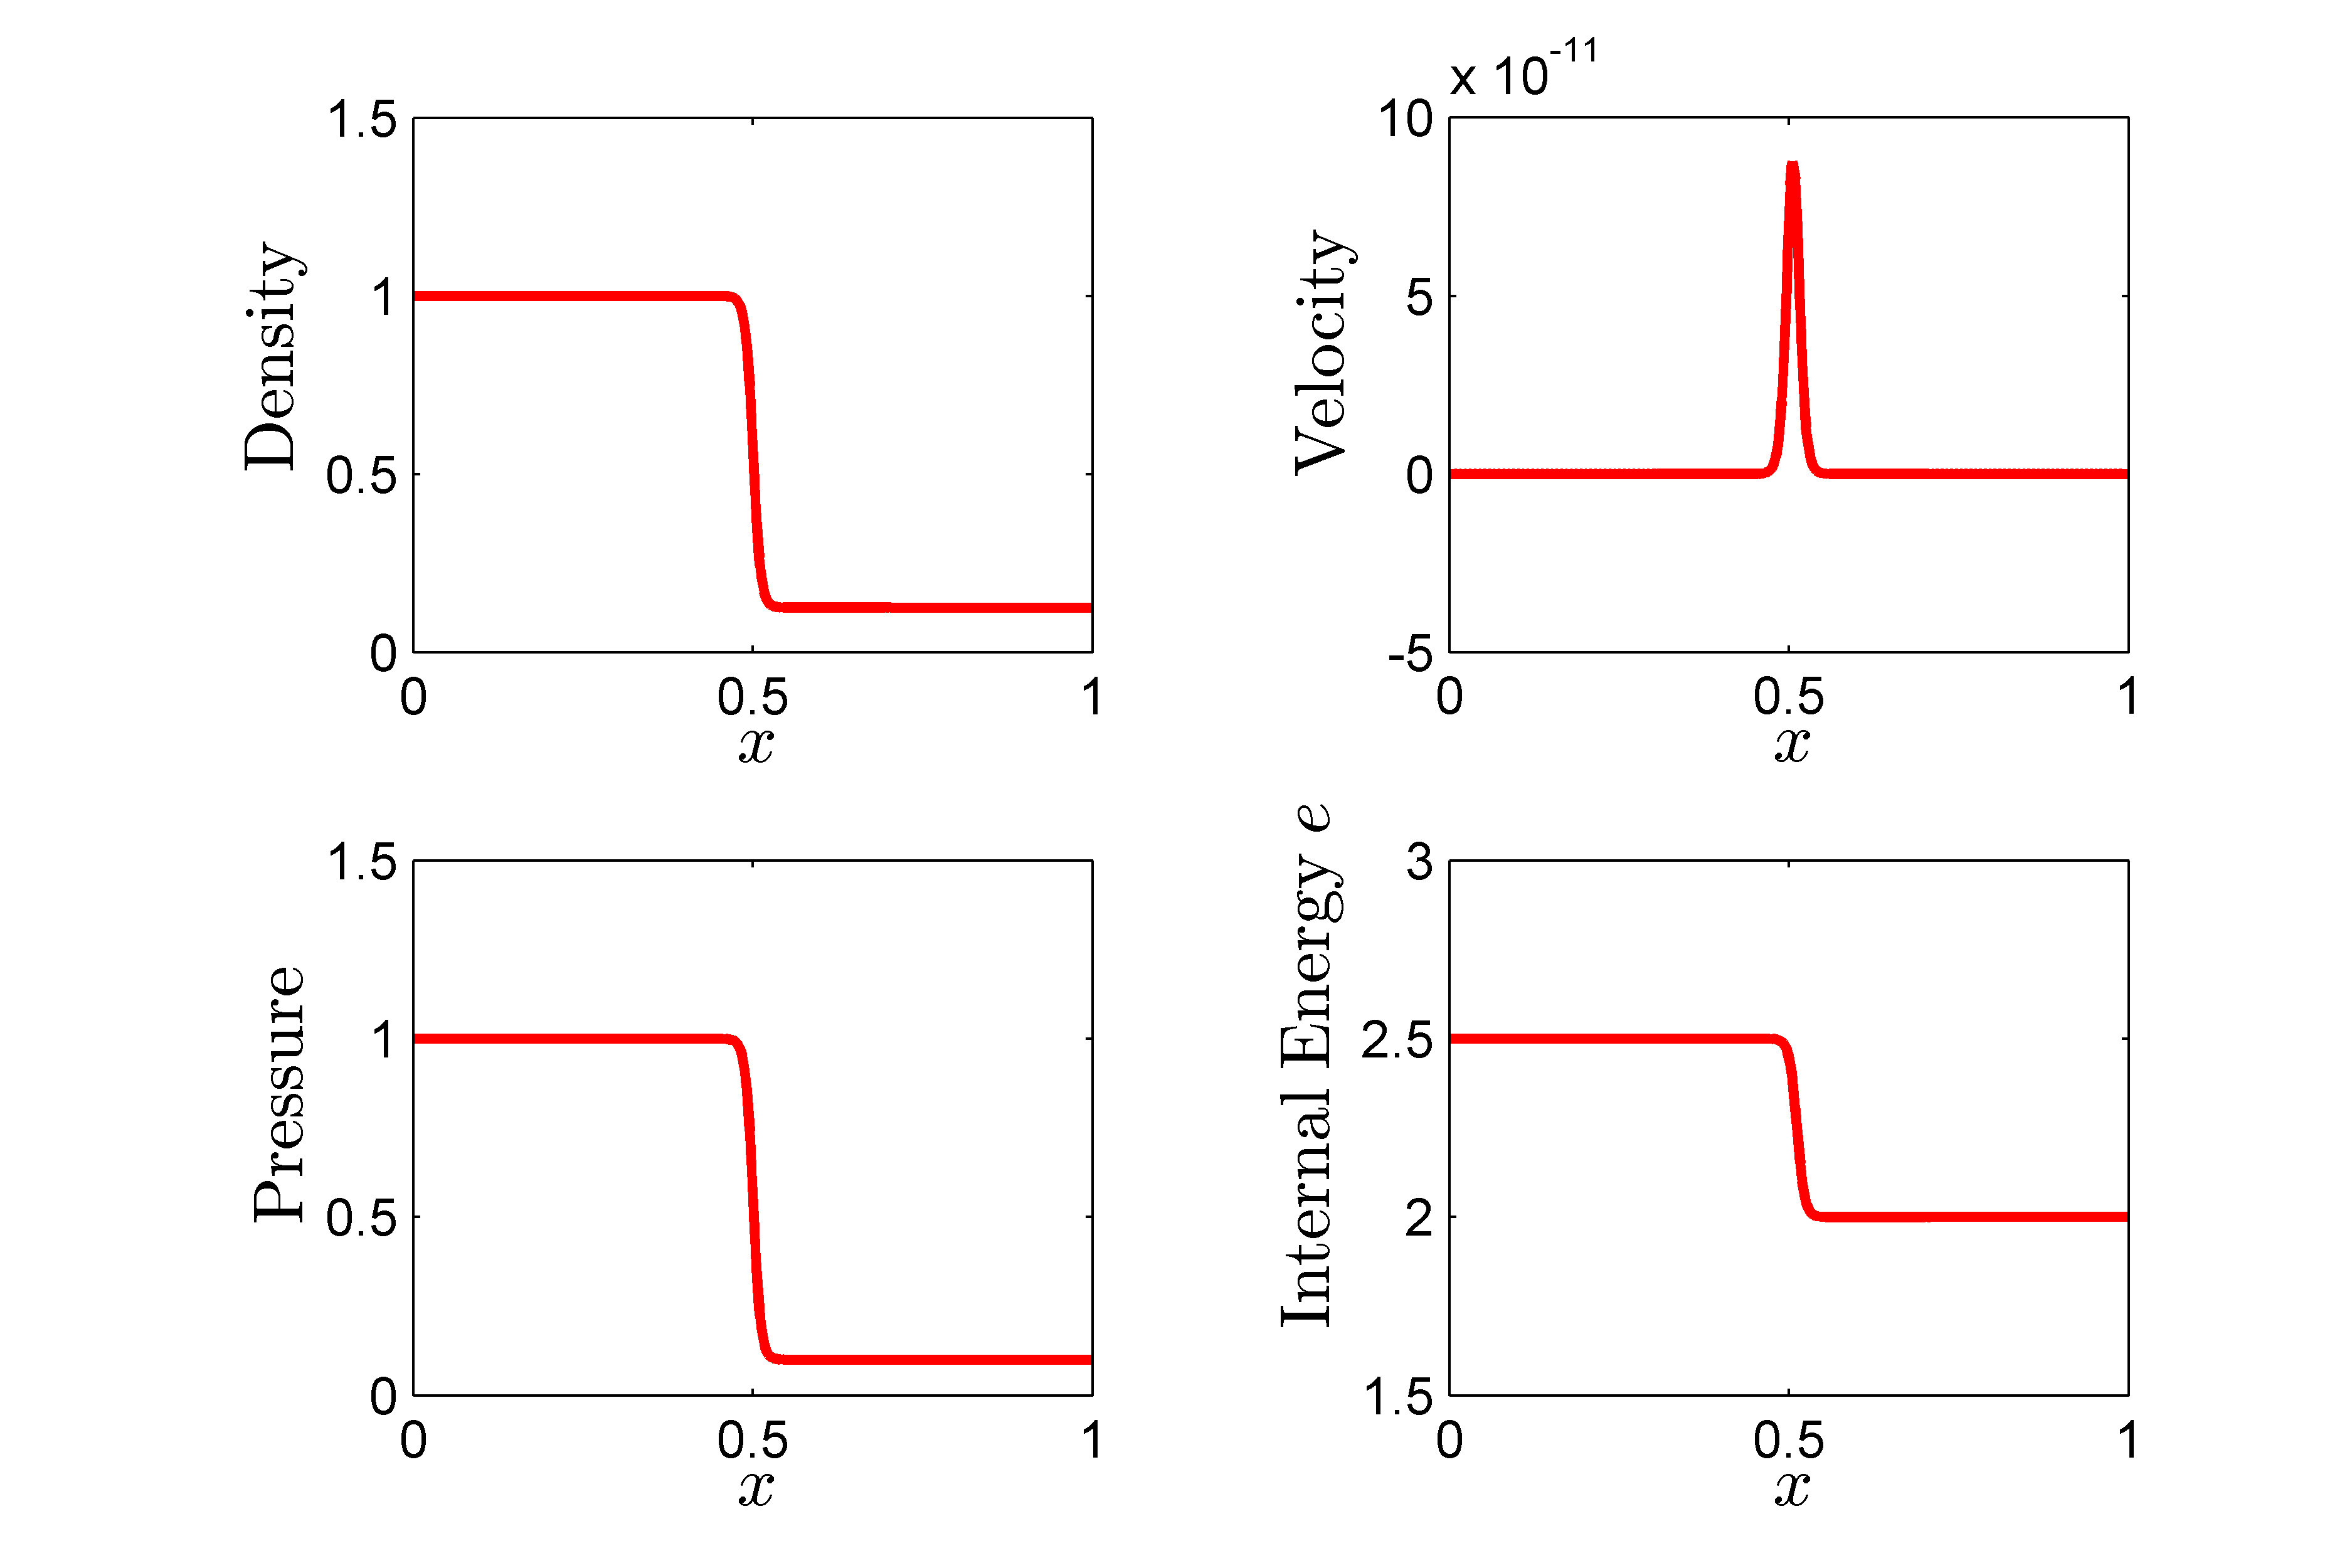
\includegraphics[width=0.525\textwidth,trim=\Ltrim cm 0cm \Rtrim cm 0cm]{\cmfrdir/Figures/Euler/Euler_shockTube_initCond.png}
  \caption{Sod's Shock Tube Problem with ``thickened'' discontinuity at $t = 0$.}
  \label{c1fr_shockTube_initCond}
\end{figure}

Figure \ref{c1fr_shockTube} shows the results to this problem at $t=0.25$ s using \gls{c1fr}. The flux used in the $0^{\mathrm{th}}$ derivative is central ($\alpha_0 = 1$ in Eqn. \eqref{eq:ifluxdef}) and the flux used in the $1^{\mathrm{st}}$ derivative is upwinded ($\alpha_1 = 0$ in Eqn. \eqref{eq:ifluxdef}). The correction functions are created with $c_1 = 1e-2$ in Eqn. \eqref{eqn:system}. The time-stepping method was \gls{rk}4, and the \gls{cfl} for the \gls{c1fr} and \gls{dg} cases was $2.5e-2$. The timestep was set to

\begin{equation}
\label{eq:cfl_cond}
\Delta t = \frac{\mathrm{\gls{cfl}} h}{|a|+|u|}
\end{equation}
where $h$ is the element size and $|a| = \sqrt{\gamma  \frac{p}{\rho}}$ is the speed of sound.

\begin{figure}
\centering
\hspace{-1.25 cm}
\centering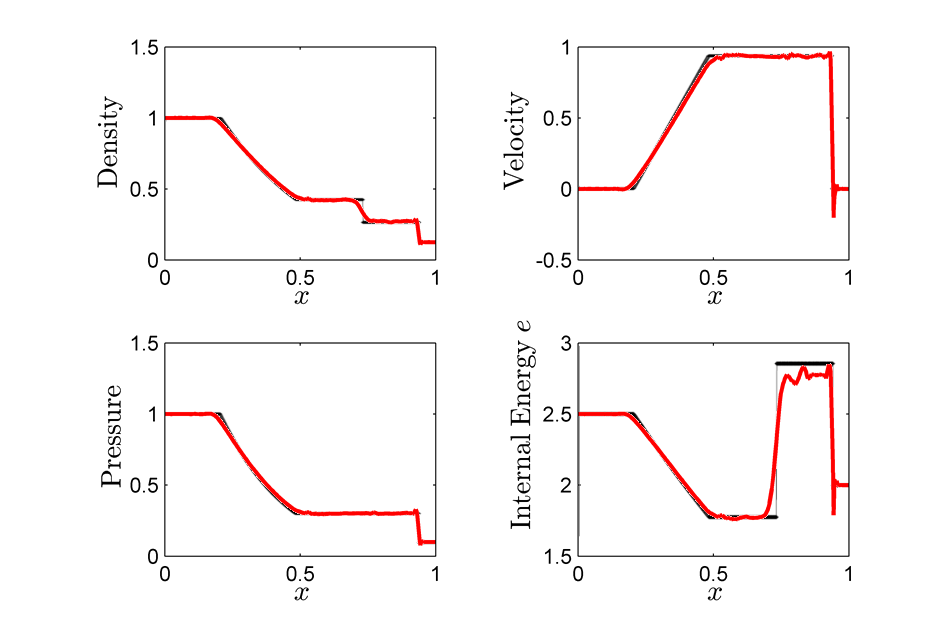
\includegraphics[width=0.2\textwidth,trim=\Ltrim cm 0cm \Rtrim cm 0cm]{\cmfrdir/Figures/Euler/Euler_shockTube.png}
  \caption{Sod's Shock Tube Problem at $t = 0.25$ solved with \gls{c1fr}. Solid black line is the exact solution to the original problem with discontinuous initial conditions. Superimposed solid red line is the solution obtained with the \gls{c1fr} scheme and ``thickened'' discontinuity in the initial conditions shown in Figure \ref{c1fr_shockTube_initCond}. $N=71, P=3,  c_1 = 1e-2, \alpha_0=1, \alpha_1 = 0, \mathrm{\gls{cfl}}=2.5e-2$}
  \label{c1fr_shockTube}
\end{figure}

The solution to the Shock Tube problem with \gls{c1fr} exhibits oscillations at the contact discontinuities, as expected. During the run of this simulation, the magnitude of these oscillation increased and decreased. The maximum value of the internal energy was not achieved. It is worth noting that slight oscillations are also present at the plateaus. This is an unexpected result, as a central flux causes large oscillations beyond the discontinuity points. It could be surmised that the upwinding of the first derivative flux acted as a limiter.

Figure \ref{c1fr_shockTube_regDG} shows the solution with regular, unfiltered, non-limited \gls{dg} with the upwinded Rusanov flux ($\alpha_0 = 0$ in Eqn. \eqref{eq:ifluxdef}).

\begin{figure}
\centering
\hspace{-1.25 cm}
\centering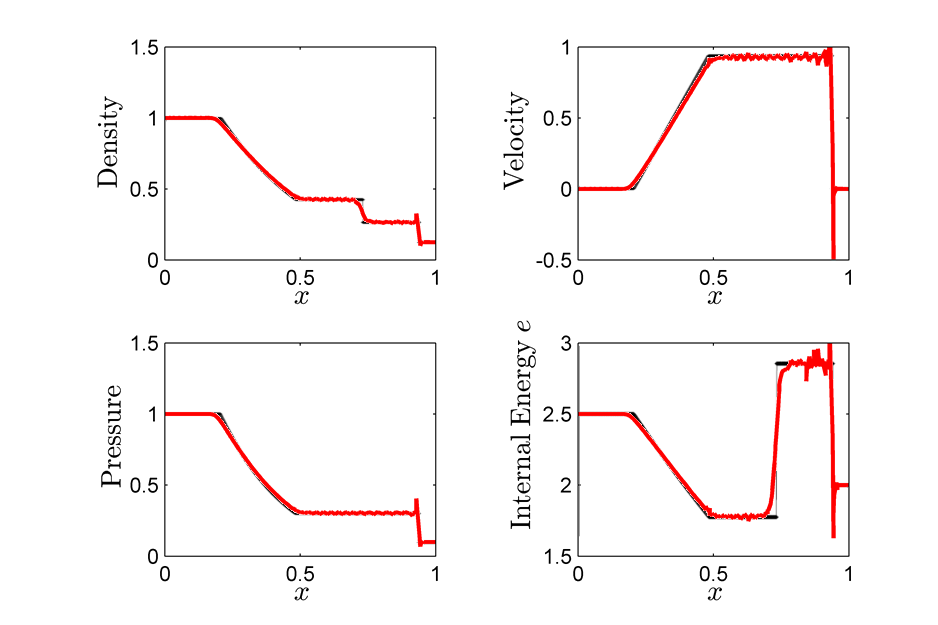
\includegraphics[width=0.2\textwidth,trim=\Ltrim cm 0cm \Rtrim cm 0cm]{\cmfrdir/Figures/Euler/Euler_shockTube_regDG.png}
  \caption{Sod's Shock Tube Problem at $t = 0.25$ solved with regular \gls{dg}. Solid black line is the exact solution to the original problem with discontinuous initial conditions. Superimposed solid red line is the solution obtained with the \gls{dg} scheme and ``thickened'' discontinuity in the initial conditions shown in Figure \ref{c1fr_shockTube_initCond}. $N=70, P=3, \alpha_0=0$}
  \label{c1fr_shockTube_regDG}
\end{figure}

The solution to the Shock Tube problem with \gls{dg} exhibits larger oscillations at the contact discontinuities than with \gls{c1fr}. The maximum value of the internal energy was achieved, albeit with very large oscillations at the discontinuity. Results by Lv et al. \cite{lv2015entropy} show that even some bounding strategies produce similar overshoot magnitudes at the discontinuities. Visible oscillations are also present at the plateaus, contrary to the results with \gls{c1fr}. This behavior is expected; \gls{dg} has been used to solve the 1-D Euler equations neatly in the presence of shocks when combined with limiters \cite{wang2015arbitrary} or filters \cite{asthana2014}. It could be surmised that the upwinding of the first derivative flux acted as a limiter.

\paragraph{123 Problem}
The 123 Problem was designed to reach conditions in which the Euler equations cannot be linearized and, hence, the Roe Flux does not provide a physical answer. It is important to note that this case is challenging for even low-order methods created specifically for the Euler equations, as seen in \cite{hudson2006review}, where the \gls{hlle} scheme \cite{einfeldt1988godunov} and \gls{ausm} \cite{liou1996sequel} are compared.
The initial conditions are, as shown in \cite{einfeldt1991godunov},
\begin{equation*}
\rho(x,0) = 1,\;\;
p(x,0) = 0.4
,\text{ and } u(x,0) = \bigg\{
\begin{tabular}{c}
$
\begin{aligned}
-2 &\text{ if } x < 0.5\\
2 &\text{ if } x \ge 0.5
\end{aligned}
$
\end{tabular}.
\end{equation*}

Figure \ref{c1fr_123_initCond} plots the initial conditions with the ``thickened'' discontinuity.

\begin{figure}
\centering
\hspace{-1.25 cm}
\centering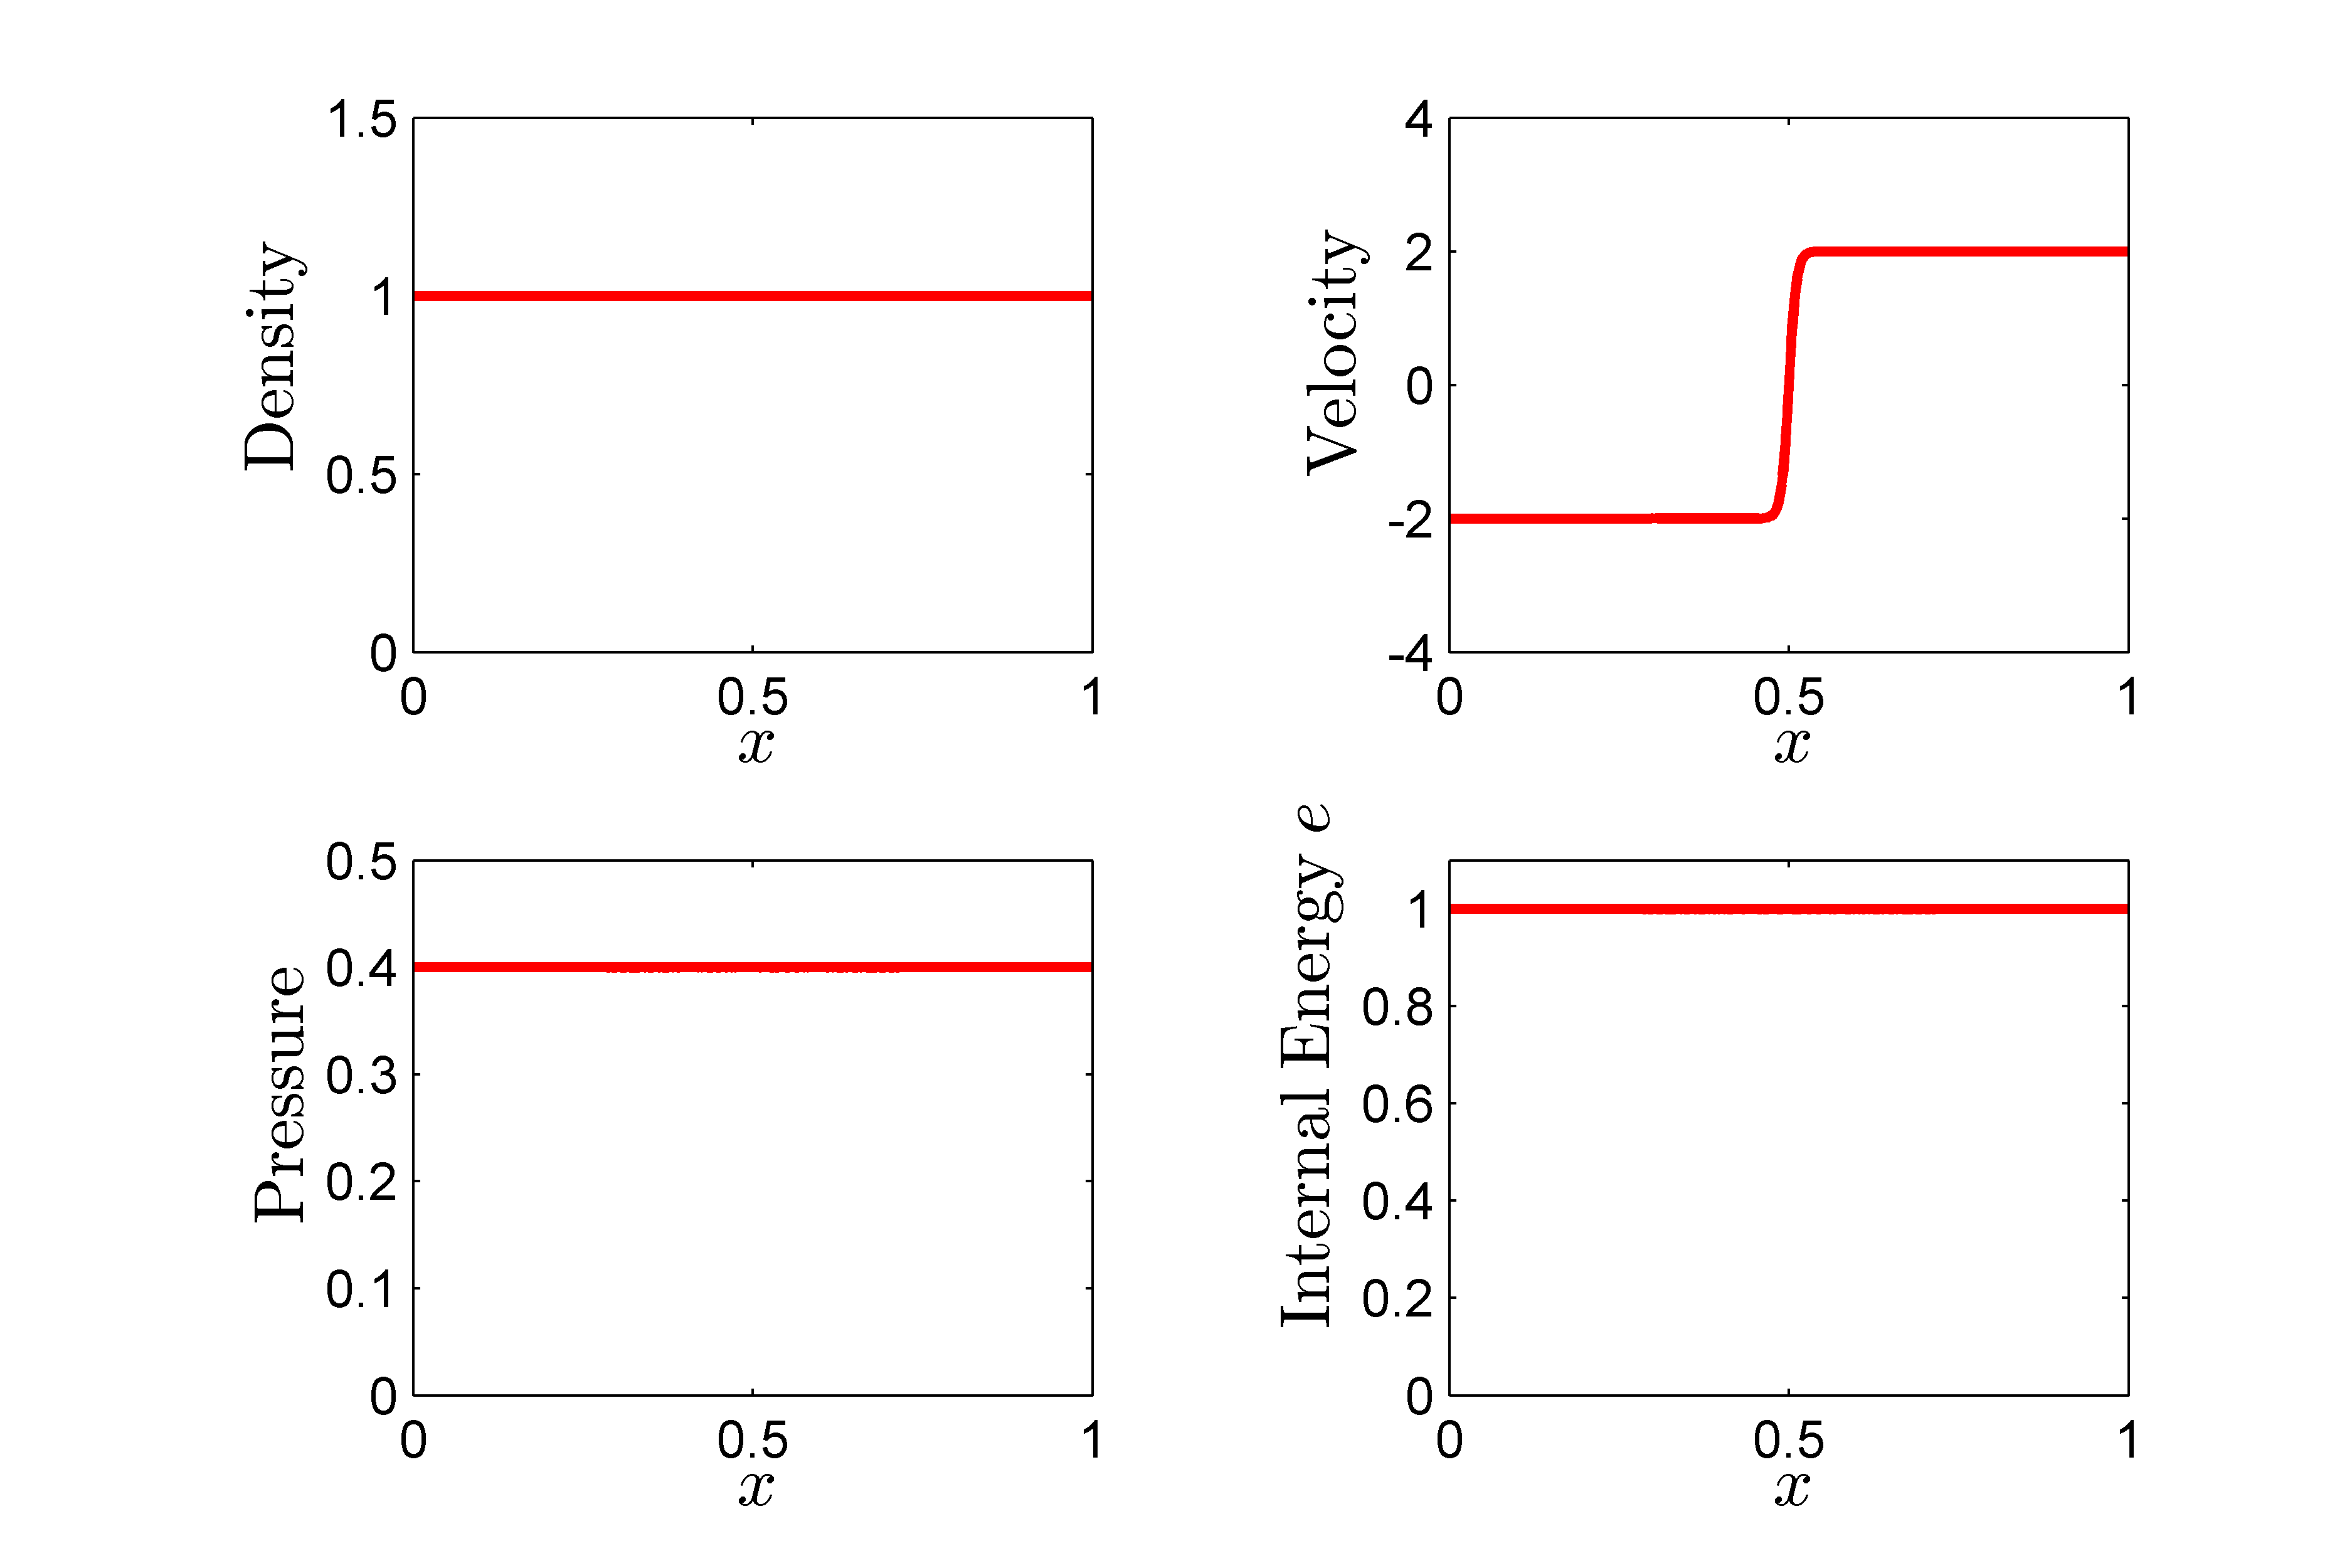
\includegraphics[width=0.525\textwidth,trim=\Ltrim cm 0cm \Rtrim cm 0cm]{\cmfrdir/Figures/Euler/Euler_123_initCond.png}
  \caption{123 Problem with ``thickened'' discontinuity at $t = 0$ solved with \gls{c1fr}. Solid black line is the exact solution to the original problem with discontinuous initial conditions. Superimposed solid red line is the solution obtained with the \gls{c1fr} scheme and ``thickened'' discontinuity in the initial conditions shown in Figure \ref{c1fr_123_initCond}. $N=71, P=3,  c_1 = 1e-2, \alpha_0=1, \alpha_1 = 0, \mathrm{\gls{cfl}}=2.5e-2$}
  \label{c1fr_123_initCond}
\end{figure}

Figure \ref{c1fr_123} shows the results at $t=0.1$ s using \gls{c1fr}. The parameters for \gls{c1fr} in this case are the same as in Section \ref{sec:shock_tube}, including the \gls{cfl}. 



Stable results with unmodified \gls{dg} could not be obtained. The reader is directed to Figure 3.4 in \cite{wang2015arbitrary} and Figure 4.3 in \cite{hudson2006review} to appreciate that accurate solutions to this problem are particularly difficult. \cite{wang2015arbitrary} needed to design fluxes for \gls{dg} to obtain a reasonable result.

The most common challenge for the schemes in the aforementioned references is that the internal energy at $x=0$ is always over-estimated. For example, as shown in \cite{hudson2006review}, \gls{hlle} overestimates $e(x=0,t=0.1)$ by $~0.1$; \gls{ausm} by $~0.8$; and \cite{wang2015arbitrary} by at least $~0.2$, even though Wang's simulations used \gls{dg} with $P=1$ (second order accurate in space). 

Given how challenging this problem is, \gls{c1fr} performed exceedingly well without the use of limiters or filters. $e(x=0,t=0.1)$ is overestimated by $~0.1$ and shows some oscillations around $x=0$. The plateau in $u(x=0, t=0.1)$ is missed (likely because of the ``thickened'' discontinuous initial conditions). This type of result suggests that \gls{c1fr} could be robust enough for flows of engineering interest.
\begin{figure}
\centering
\hspace{-1.25 cm}
\centering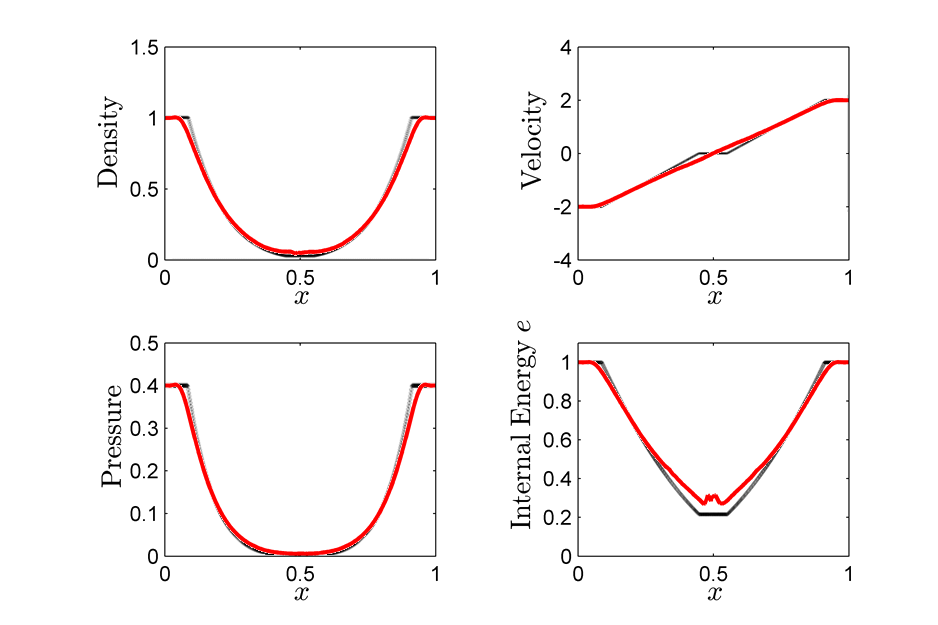
\includegraphics[width=0.2\textwidth,trim=\Ltrim cm 0cm \Rtrim cm 0cm]{\cmfrdir/Figures/Euler/Euler_123.png}
  \caption{123 problem at $t = 0.1$. Solid black line is the exact solution. Superimposed solid red line is the solution obtained with the \gls{c1fr} scheme.}
  \label{c1fr_123}
\end{figure}